\documentclass[a0]{sciposter}
\usepackage{graphicx}
\usepackage{color}
\usepackage{multicol}
\usepackage{url}
\usepackage{ragged2e}
\usepackage{watermark}
\usepackage{fancyvrb}
\usepackage{amstext}

\newcommand{\figfigure}[2]{%
  \includegraphics[width=#1]{#2}
}

\setlength{\columnseprule}{.5pt}
\setlength{\parskip}{12pt}

\title{
  The \textcolor{red}{igraph} platform for network science}
\author{
  G\'abor Cs\'ardi$^{\scriptscriptstyle 1,2}$ and 
  Tam\'as Nepusz$^{\scriptscriptstyle 1,3}$}
\institute{\mbox{}$^1$Department of Biophysics, 
  Research Institute for Particle and Nuclear Physics \\
  of the Hungarian Academy of Sciences,
  Budapest, Hungary. \\
  \mbox{}$^2$Center for Complex Systems Studies, Kalamazoo College,
  Kalamazoo, MI, USA. \\
  \mbox{}$^3$Dept. of Measurement and Information Systems, Budapest
  University of Technology and Economics, Budapest, Hungary.
}
\email{csardi@rmki.kfki.hu \& ntamas@rmki.kfki.hu}
\leftlogo{RMKI-BME}
\rightlogo{CCSS}

\begin{document}

\watermark{\includegraphics[angle=-90,width=\textwidth]{karate3d}}

\maketitle

\begin{multicols}{3}

\section{Features}

\begin{itemize}
\item Efficient and simple graph representation. Storing a graph needs
  32 bytes per edge and 16 bytes per vertex.
\item Efficient implementation. The current state of the art
  algorithms are implemented (if not that is considered as a bug).
\item Portable C (and some C++) code, works on most platforms:
  Linux flavours, MS Windows variations, Mac OSX, Solaris, etc.
\item Wide variety of graph algorithms: random and regular graph
  structures, centrality measures, shortest paths, 2D and 3D graph
  layouts, graph motifs, cliques, network flows and cuts, community
  structure detection, etc.
\item Interfaces from GNU R and Python, other interfaces can be added
  without too much hassle.
\item Interactive and non-interactive, 2D and 3D
  visualization from R and Python.
\item Graph, vertex and edge attributes, like edge weights, vertex
  colors and other parameters for plotting.
\item Various import and export file formats: GraphML, GML, Pajek,
  simple edge list, etc.
\item Well documented.
\item Open source and completely free for non-commercial and
  commercial use.
\end{itemize}

\section{Architecture}

Simple and flexible layered architecture.
Modules interact via well-defined interfaces and 
can be replaced individually without breaking other parts.

\begin{center}
\figfigure{\columnwidth}{arch}
\end{center}

\section{Examples and Screenshots}

% \vspace{20pt}\hrule\vspace{20pt}
% \centerline{\bf Python interface screeshot}
% \vspace{20pt}\hrule\vspace{20pt}

% \begin{center}
% 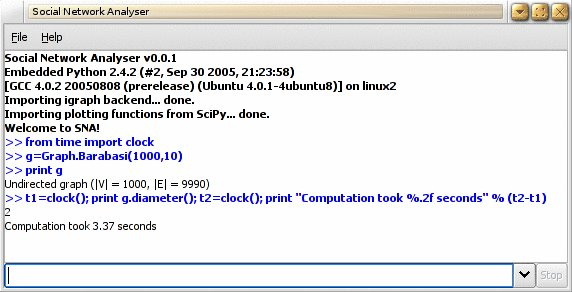
\includegraphics[width=\columnwidth]{sna_screenshot}
% \end{center}

% \columnbreak

\vspace{20pt}\hrule\vspace{20pt}
\centerline{\bf Eigenvector based community structure}
\vspace{20pt}\hrule\vspace{20pt}

\begin{Verbatim}[fontsize=\small,numbers=left]
g <- read.graph(
    "http://www.rmki.kfki.hu/~csardi/karate.gml", 
    format="GML")

community.newman <- function(g) {
  d <- degree(g)
  B <- get.adjacency(g)-outer(d, d, function(x,y) 
                                    x*y/2/ecount(g))
  diag(B) <- 0
  eigen(B)$vectors[,1]
}

mem <- community.newman(g)
V(g)$color <- ifelse(mem < 0, "blue", "green")
V(g)$size <- abs(mem) * 35 ; E(g)$color <- "darkblue"
E(g) [ V(g)[mem>=0] %--% V(g)[mem>=0] ]$color <- 
     "darkgreen"
E(g) [ V(g)[mem< 0] %--% V(g)[mem>=0] ]$color <- "red"
tkplot(g, layout=layout.fruchterman.reingold,
       vertex.label.dist=1)
\end{Verbatim}

\begin{center}
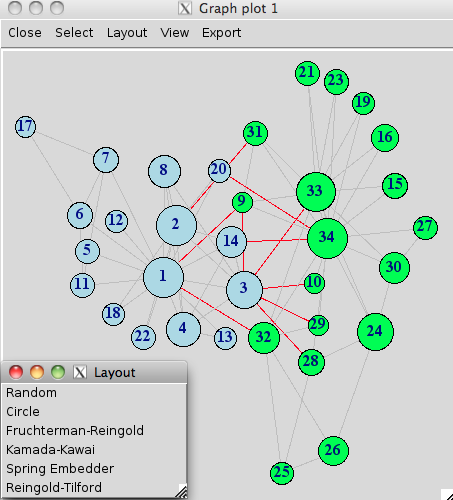
\includegraphics[width=0.7\columnwidth]{tkplot}
\end{center}

\vspace{20pt}\hrule\vspace{20pt}
\centerline{\bf Diameter of a scale-free graph}
\vspace{20pt}\hrule\vspace{20pt}

\begin{Verbatim}[fontsize=\small,numbers=left]
g <- barabasi.game(100, directed=FALSE)
d <- get.diameter(g)
E(g)$color <- "SkyBlue2"
E(g)$width <- 1
E(g, path=d)$color <- "red"
E(g, path=d)$width <- 2
V(g)$label.color <- V(g)$color  <- "blue"
V(g)[ d ]$label.color <- V(g)[ d ]$color <- "red"
plot(g, layout=layout.fruchterman.reingold, 
     vertex.label.dist=0.6, vertex.size=3)
title(main="Diameter of small scale-free graph",
      xlab="created by igraph 0.4")
\end{Verbatim}

\begin{center}
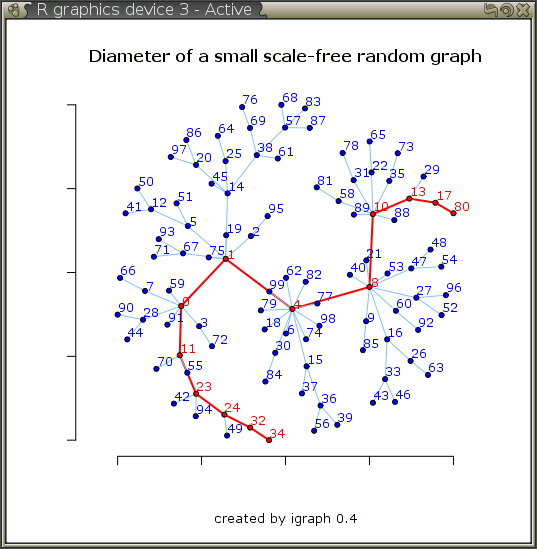
\includegraphics[width=0.7\columnwidth]{diameter}
\end{center}

\vspace{20pt}\hrule\vspace{20pt}
\centerline{\bf Some degree distributions}
\vspace{20pt}\hrule\vspace{20pt}

\begin{Verbatim}[fontsize=\small,numbers=left]
g <- barabasi.game(100000)
d <- degree(g, mode="in")
dd <- degree.distribution(g, mode="in", cumul=TRUE)
alpha <- power.law.fit(d, xmin=20)
plot(dd, log="xy", xlab="degree", 
     ylab="cumulative frequency",
     col=1, main="Nonlinear preferential attachment")
lines(10:500, 10*(10:500)^(-coef(alpha)+1))

powers <- c(1.0, 0.9, 0.8, 0.7, 0.6)
for (p in seq(powers[-1])) {
  g <- barabasi.game(100000, power=powers[p+1])
  dd <- degree.distribution(g, mode="in", cumul=TRUE)
  points(dd, col=p+1, pch=p+1)
}
legend(1,1e-5, powers, col=1:5, pch=1:5, yjust=0, lty=0)
\end{Verbatim}

\begin{center}
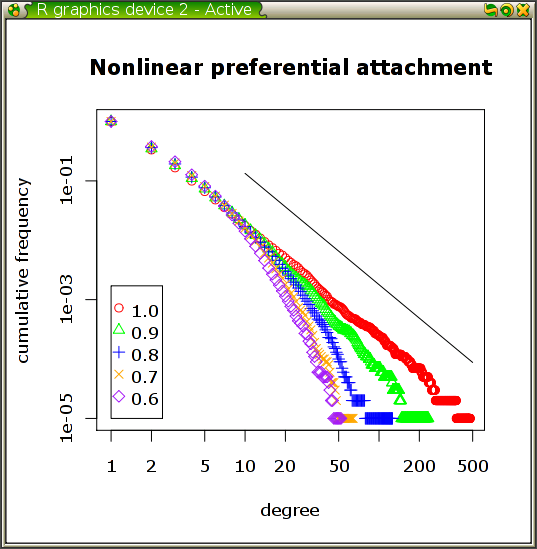
\includegraphics[width=0.7\columnwidth]{degreedist}
\end{center}

\columnbreak
\vspace{20pt}\hrule\vspace{20pt}
\centerline{\bf Page Rank in Python}
\vspace{20pt}\hrule\vspace{20pt}

\begin{Verbatim}[fontsize=\small,numbers=left]
from igraph import *
from copy import copy

def pagerank(g, damping=0.85, epsilon=0.001, iters=100):
  pageranks = [1-damping] * g.vcount()
  outlinks = g.degree(type=OUT)
  mindiff = epsilon
  newprs = [0] * g.vcount()
    
  while mindiff >= epsilon and iters > 0:
    iters = iters - 1
    for n in range(g.vcount()):
      neis = g.neighbors(n, IN)
      pr = 0.0
      if len(neis) > 0:
        for n2 in neis: pr = pr+pageranks[n2]/outlinks[n2]
        pr = pr*damping
      newprs[n] = pr+1-damping
 
    mindiff = min([abs(newprs[n]-pageranks[n]) for n 
              in range(g.vcount())])
    pageranks = copy(newprs)
	
  return pageranks
\end{Verbatim}

\vspace{20pt}\hrule\vspace{20pt}
\centerline{\bf 3D visualization in Python}
\vspace{20pt}\hrule\vspace{20pt}

\begin{center}
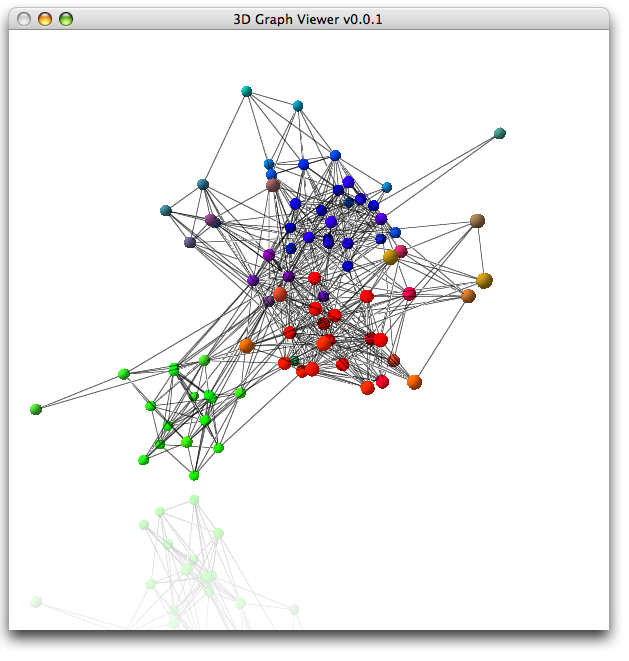
\includegraphics[width=0.7\columnwidth]{python3d-2}
\end{center}

\vspace{20pt}\hrule\vspace{20pt}
\centerline{\bf Dijkstra's shortest path algorithm}
\vspace{20pt}\hrule\vspace{20pt}

\begin{Verbatim}[fontsize=\small,numbers=left]
wsp <- function(g, source, weights=E(g)$weight) {
  vc <- vcount(g)
  res <- numeric(vc)
  visited <- logical(vc)
  visited[source+1] <- TRUE
  while (any(!visited)) {
    edges <-  E(g) [ V(g)[visited] %--% V(g)[!visited] ]
    ft <- get.edges(g, edges)
    weig <- weights[ edges+1 ] +
            res[ft[,1]+1] + res[ft[,2]+1]
    minw <- which.min(weig)
    ft <- ft[minw,]
    if (visited[ft[2]+1]) ft <- rev(ft)
    res[ft[2]+1] <- weig[minw]
    visited[ ft+1 ] <- TRUE
  }
  res
}
\end{Verbatim}

\vspace{20pt}\hrule\vspace{20pt}
\centerline{\bf Weighted transitivity}
\vspace{20pt}\hrule\vspace{20pt}

\[ 
  c(i)=\frac{\mathbf{A}^3_{ii}}{(\mathbf{A1A})_{ii}} \qquad
  c_w(i)=\frac{\mathbf{W}^3_{ii}}{(\mathbf{WW_{\text{max}}W})_{ii}}
\]

\begin{Verbatim}[fontsize=\small,numbers=left]
wtrans <- function(g) {
  W <- get.adjacency(g, attr="weight")
  WM <- matrix(max(W), nrow(W), ncol(W))
  diag(WM) <- 0
  diag( W %*% W %*% W ) / diag( W %*% WM %*% W)
}
\end{Verbatim}

\section{Where to get it?}
\centerline{\bf\LARGE \url{http://igraph.sf.net}}

\end{multicols}

\enlargethispage{2cm}
\vfill
\hrule
\vfill
\centerline{\small NetSci 2007 International Workshop and Conference
  on Network Science}
\vfill

\end{document}
